\chapter{Plano de gerenciamento das mudanças} % Ver http://www.pmtech.com.br/artigos/PlanosProjeto/Plano%20de%20Projeto%20Modelo%20V2%200.pdf
\label{ch:change-management-plan}

\section{Objetivo}

No contexto deste projeto mudanças podem surgir por diversos motivos. Os fatores que originam estas mudanças podem ser:

\begin{itemize}
	\item Mudanças na legislação.
	\item Mudanças solicitadas pelo patrocinador para incrementar ou reduzir funcionalidades nas soluções desenvolvidas.
	\item Mudanças solicitadas pelo patrocinador para responder as necessidades ou direcionamento de negócios.
	\item Mudanças solicitadas pela equipe do projeto a fim de atender as particularidades técnicas que podem surgir durante o desenvolvimento do projeto.
\end{itemize}

Estas alterações impactam diretamente no escopo, tempo e qualidade do projeto. A fim de estabelecer procedimentos claros e formais, se faz necessário a criação do plano de gerenciamento das mudanças. Neste plano estão definidos os procedimentos para tratar as mudanças que podem ser aprovadas.

\section{Priorização integrada de mudanças}
\label{sec:integrated-change-priorization}

Ao surgir uma necessidade de mudança no projeto a dependência entre tarefas deve ser considerada, para isso utiliza-se um sistema contendo três níveis de classificação conforme descrito a seguir:

\begin{description}
	\item[Prioridade Baixa:] Mudanças de prioridade baixa não requerem uma ação imediata. São mudanças que podem alterar as entregas intermediárias sem que se comprometa o prazo final de entrega do projeto. Os prazos das entrega intermediárias devem ser revisados durante a reunião do CCM. Não requer autorização do patrocinador na maioria dos casos.
	\item[Prioridade Média:] Mudanças de prioridade média são mudanças que impactam em prazo e custo e requerem ação imediata do gerente do projeto para recuperação do mesmo. Para isso o gerente pode utilizar medidas como horas extras ou reservas gerenciais.
	\item[Prioridade Alta:] Mudanças de prioridade alta são mudanças de alto impacto no projeto e com solução de difícil identificação. Este tipo de mudança requer uma ação imediata por parte do gerente do projeto, que deve acionar imediatamente o patrocinador para análise e discussão sobre ações a serem tomadas.
\end{description}

Mudanças que não geram impacto significativo no projeto não serão classificadas de acordo com estas prioridades, poderão ser apenas gerenciadas e controladas pelo gerente do projeto.

\section{Sistema de controle integrado das mudanças}
\label{sec:change-control-system}

As necessidades de mudança que surgirem no projeto deverão ser tratadas de acordo com o fluxo de controle integrado de mudanças visto na figura \ref{img:change-control-flow}.

\begin{figure}[h]
	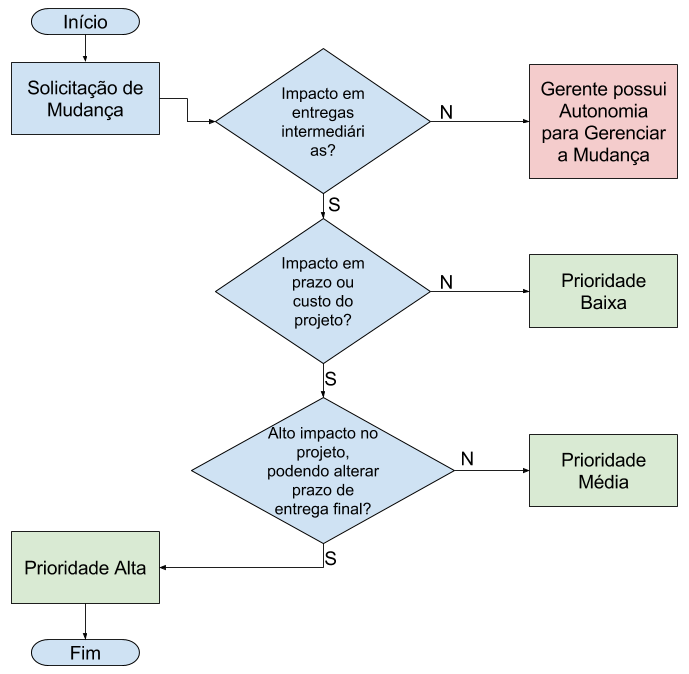
\includegraphics[width=\textwidth]{images/fluxo-controle-mudancas}
	\label{img:change-control-flow}
	\caption{Fluxo de controle das mudanças.}
\end{figure}

\section{Comitê de controle de mudanças}

Será criado um comitê executivo, composto pelo patrocinador, pelo gerente de projetos, pelo engenheiro de software, pelo arquiteto de soluções e pelo engenheiro eletricista, totalizando cinco participantes. Esse comitê será responsável pela análise e aprovação das mudanças.

O processo de decisão do comitê será baseado em consenso, tendo o patrocinador o direito de vetar e aprovar decisões caso o consenso não seja obtido.

\section{Início das mudanças}

\subsection{Autorização}

O gerente de projeto e o patrocinador serão os responsáveis por iniciar o processo do pedido de mudanças.

\subsection{Processo de início das mudanças}

Qualquer membro da equipe do projeto, o patrocinador e outros funcionários da empresa poderão detectar uma necessidade de mudança. Em quaiquer dos casos o gerente de projeto será responsável pelo recebimento e orientação no uso do formulário de requisição de mudança, podendo ocorrer de o gerente de projeto realizar todo o processo para requisição de mudança.

Todas as solicitações de mudança deverão ser submetidas por escrito ou através de e-mail utilizando o fomrulário para requisição de mudança (ver apêndice \ref{ch:change-request-form}), conforme descrito no plano de comunicações do projeto.

\section{Avaliação das mudanças}

A classificação e análise das solicitações de mudança serão realizadas durante a reunião do CCM. Caso o gerente de projeto identifique mudanças de alto impacto no projeto uma reunião extraordinária do CCM deverá ser convocada imediatamente.

\section{Aprovação das mudanças}

Mudanças de alto impacto no projeto deverão ser aprovadas pelo patrocinador do projeto.

\section{Implantação das mudanças}

O gerente de projeto será responsável por atualizar os planos de projeto, tomando as ações necessárias para implantar as mudanças nos prazos acordados.

\section{Registros}

O gerente de projeto será responsável pelo registro de todas mudanças apresentadas. 

\section{Controle de Versão}

\begin{table}[H]
	\begin{tabularx}{\textwidth}{| c | c | X | X |}
		\hline
		\textbf{Versão} & \textbf{Data} & \textbf{Autor}      & \textbf{Notas de Revisão} \\
		\hline
		1                &               & \projectManagerName{} & Criação do documento     \\
		\hline
	\end{tabularx}
	\centering
\end{table}

\section{Aprovações}

\begin{table}[H]
	\begin{tabularx}{\textwidth}{| c | c | X | c |}
		\hline
		\textbf{Função}  & \textbf{Nome}       & \textbf{Assinatura}      & \textbf{Data} \\
		\hline
		Patrocinador       & \projectSponsorName{} & \projectSponsorSignature{} &               \\
		\hline
		Gerente de projeto & \projectManagerName{} & \projectManagerSignature{} &               \\
		\hline
	\end{tabularx}
	\centering
\end{table}